\documentclass[submit]{harvardml}

% FDV: Update front matter -- years, dates, references to book sections, etc.
\course{CS181-S22}
\assignment{Assignment \#5}
\duedate{11:59pm EST, April 8, 2021}

\newcommand{\attr}[1]{\textsf{#1}}
\usepackage[OT1]{fontenc}
\usepackage[colorlinks,citecolor=blue,urlcolor=blue]{hyperref}
\usepackage[pdftex]{graphicx}
\usepackage{subfig}
\usepackage{framed}
\usepackage{fullpage}
\usepackage{amsmath}
\usepackage{amssymb}
\usepackage{color}
\usepackage{todonotes}
\usepackage{listings}
\usepackage{common}
\usepackage{bm}
\usepackage{enumitem}
\usepackage{tikz}
\usetikzlibrary{positioning,shapes,arrows}
\usepackage{xifthen}
\usepackage{pythonhighlight}
\usepackage{soul}

\usepackage[mmddyyyy,hhmmss]{datetime}

\definecolor{verbgray}{gray}{0.9}

\lstnewenvironment{csv}{
  \lstset{backgroundcolor=\color{verbgray},
  frame=single,
  framerule=0pt,
  basicstyle=\ttfamily,
  columns=fullflexible}}{}

\begin{document}


\begin{center}
{\Large Homework 5: EM with Mixtures, PCA, and Graphical Models}\\
\end{center}

This homework assignment will have you work with EM for mixtures, PCA,
and graphical models. We encourage you to read sections 9.4 and 8.2.5 of the course textbook.

Please type your solutions after the corresponding problems using this
\LaTeX\ template, and start each problem on a new page.

Please submit the \textbf{writeup PDF to the Gradescope assignment `HW5'}. Remember to assign pages for each question.

Please submit your \textbf{\LaTeX\ file and code files to the Gradescope assignment `HW5 - Supplemental'}. 


\newpage
\begin{problem}[Expectation-Maximization for Gamma Mixture Models, 25pts]

In this problem we will explore expectation-maximization for a Categorical-Gamma Mixture model.

Let us suppose the following generative story for an observation $x$: first one of $K$ classes is randomly selected, and then the features $x$ are sampled according to this class. If $$z \sim \operatorname{Categorical}(\btheta)$$ indicates the selected class, then $x$ is sampled according to the class or ``component'' distribution corresponding to $z$. (Here, $\btheta$ is the mixing proportion over the $K$ components: $\sum_k \theta_k = 1$ and $ \theta_k > 0$). In this problem, we assume these component distributions are gamma distributions with shared shape parameter but different rate parameters: $$x | z \sim \operatorname{Gamma}(\alpha, \beta_k).$$

In an unsupervised setting, we are only given a set of observables as our training dataset: $\mathcal D = \{x_n\}_{n=1}^N$. The EM algorithm allows us to learn the underlying generative process (the parameters $\btheta$ and $\{\beta_k\}$) despite not having the latent variables $\{z_n\}$ corresponding to our training data.

\vspace{2em}

\begin{enumerate}

  \item \textbf{Intractability of the Data Likelihood} We are
    generally interested in finding a set of parameters $\beta_k$ that
    maximizes the likelihood of the observed data: $$\log
    p(\{x_n\}^N_{n=1}; \btheta, \{\beta_k\}^K_{k = 1}).$$ Expand the data
    likelihood to include the necessary sums over observations
    $x_n$ and to marginalize out the latents
    $\boldz_n$. Why is optimizing this likelihood directly
    intractable?

\item \textbf{Complete Data Log Likelihood} The complete dataset
  $\mathcal D = \{(x_n, \boldz_n)\}_{n=1}^N$ includes latents $\boldz_n$. Write
  out the negative complete data log likelihood: $$\mcL(\btheta, \{\beta_k\}^K_{k=1}) =  -\log p(\mathcal D; \btheta, \{\beta_k\}^K_{k=1}).$$

  Apply the power trick and simplify your expression using indicator elements $z_{n
  k}$.\footnote{The ``power trick'' is used when terms in a PDF are raised to the power of indicator components of a one-hot vector.  For example, it allows us to rewrite $p(\boldz_n ;  \btheta) = \prod_k \theta_k^{z_{nk}}$.} Notice that optimizing this loss is now computationally tractable if we know $\boldz_n$.

  (Continued on next page.)

\end{enumerate}

\end{problem}

\newpage


\begin{framed}
\noindent\textbf{Problem 1} (cont.)\\
\begin{enumerate}
\item[3.] \textbf{Expectation Step} Our next step is to introduce a
  mathematical expression for $\boldq_n$, the posterior over the
  hidden component variables~$\boldz_n$ conditioned on the observed data
  $x_n$ with fixed parameters.
That is:
  \begin{align*}
    \textbf{q}_n &= \begin{bmatrix}
      p(\boldz_n =\boldC_1| x_n; \btheta, \{ \beta_k \}^K_{k=1}) \\
      \vdots \\
      p(\boldz_n =\boldC_K| x_n; \btheta, \{ \beta_k \}^K_{k=1})
    \end{bmatrix}.
  \end{align*}
  %
%
  Write down and simplify the expression for
  $\boldq_n$.  Note that because the $\boldq_n$ represents the
  posterior over the hidden categorical variables $\boldz_n$, the
  components of vector $\boldq_n$ must sum to 1.
  The main work is to find an expression for $p(\boldz_n|x_n; \btheta, \{\beta_k\}^K_{k=1})$  for any choice of $\boldz_n$; i.e., for any 1-hot encoded $\boldz_n$. With this, you can then construct the different components that make up the vector $\boldq_n$.
  
\item[4.] \textbf{Maximization Step}
Using the~$\boldq_n$ estimates from the Expectation Step, derive an update for maximizing the expected complete data log likelihood in terms of $\btheta$ and $\{ \beta_k \}^K_{k=1}$.

\begin{enumerate}
    \item Derive an expression for the expected complete data log likelihood using $\boldq_n$.
    \item Find an expression for $\btheta$ that maximizes this expected complete data log likelihood. You may find it helpful to use Lagrange multipliers in order to enforce the constraint $\sum \theta_k = 1$. Why does this optimal $\btheta$ make intuitive sense?
    \item Find an expression for $\beta_k$ that maximizes the expected complete data log likelihood.  Why does this optimal $\beta_k$  make intuitive sense?
\end{enumerate}
    
\item[5.] Suppose that this had been a classification problem. That is,
  you were provided the ``true'' components $\boldz_n$ for each
  observation $x_n$,
  and you were going to perform the classification by
  inverting the provided generative model (i.e. now you're predicting $\boldz_n$ given $x_n$). Could you reuse any of
  your derivations above to estimate the parameters of the model?
  

\item[6.] Finally, implement your solution in \texttt{p1.ipynb} and attach the final plot below.

{\bfseries You will recieve no points for code not included below.}
\end{enumerate}
  
\end{framed}

\newpage
\subsection*{Solution}

\begin{enumerate}
  \item We can begin by writing down the likelihood of the data, given the parameters:
  \begin{align*}
      p(\{x_n\}^N_{n=1}; \btheta, \{\beta_k\}^K_{k = 1}) &= \prod_{n=1}^N p(x_n; \btheta, \{\beta_k\}^K_{k = 1})\\
      &= \prod_{n=1}^N \sum_{k=1}^K p(x_n; \btheta, \{\beta_k\}^K_{k = 1}) p(z_n = C_k; \btheta_k)
  \end{align*}
  Using the Law of Total Probability (LOTP), we discover that the likelihood of each individual data point is equal to the gamma distribution multiplied by the categorical distribution summed over every class. Thus, the log likelihood is given by:
  \begin{align*}
      \log p(\{x_n\}^N_{n=1}; \btheta, \{\beta_k\}^K_{k = 1}) &= \log \left[\prod_{n=1}^N \sum_{k=1}^K p(x_n; \btheta, \{\beta_k\}^K_{k = 1}) p(z_n = C_k; \btheta_k)\right]\\
      &= \log \left[\prod_{n=1}^N \sum_{k=1}^K \operatorname{Gamma}(\alpha, \beta_k) \cdot \btheta_k\right]\\
      &= \sum_{n=1}^N \log \left[ \sum_{k=1}^K \operatorname{Gamma}(\alpha, \beta_k) \cdot \btheta_k\right]
  \end{align*}
  Optimizing this log likelihood is intractable because we cannot easily optimize the log of the sum, even though we can adeptly optimize a sum of logs.
  
  \item
  We can expand the negative complete data log likelihood using LOTP:
  \begin{align*}
      \mcL(\btheta, \{\beta_k\}^K_{k=1}) &=  -\log p(\mathcal D; \btheta, \{\beta_k\}^K_{k=1})\\
      &=  -\log \left[\prod_{n=1}^N p(x_n; \btheta, \{\beta_k\}^K_{k=1})\right]\\
      &=  -\sum_{n=1}^N \log \left[p(x_n; \btheta, \{\beta_k\}^K_{k=1})\right]\\
      &=  -\sum_{n=1}^N \log \left[\prod_{k=1}^K p(x_n | z_n = C_k; \btheta, \{\beta_k\}^K_{k=1}) p(z_n = C_k; \btheta_k)\right]\\
      &=  -\sum_{n=1}^N \left(\log \left[\prod_{k=1}^K p(x_n | z_n = C_k; \btheta, \{\beta_k\}^K_{k=1})\right] + \log \left[\prod_{k=1}^K p(z_n = C_k; \btheta_k)\right]\right)
  \end{align*}
  Applying the power trick, where $z_{nk}$ is the indicator that $x_n$ is sampled from class $k$ ($C_k$), we get:
  \begin{align*}
      \mcL(\btheta, \{\beta_k\}^K_{k=1}) &= -\sum_{n=1}^N \left(\log \left[\prod_{k=1}^K p(x_n; \btheta, \{\beta_k\}^K_{k=1})^{z_{nk}}\right] + \log \left[\prod_{k=1}^K\btheta_k^{z_{nk}}\right]\right)\\
      &= -\sum_{n=1}^N \left(\sum_{k=1}^K z_{nk}\left( \log \left[p(x_n; \btheta, \{\beta_k\}^K_{k=1})\right] + \log \left[\btheta_k\right]\right)\right)\\
      &= -\sum_{n=1}^N \left(\sum_{k=1}^K z_{nk}\log \left[\operatorname{Gamma}(\alpha, \beta_k) \cdot \btheta_k\right]\right)
  \end{align*}
  
  \item
  First, find $\textbf{q}_{nk} = p(\boldz_n =\boldC_k| x_n; \btheta, \{ \beta_k \}^K_{k=1})$. Using Bayes' Rule and LOTP in the denominator, we get:
  \begin{align*}
      \textbf{q}_{nk} &= \frac{p(x_n | \boldz_n =\boldC_k; \btheta, \{ \beta_k \}^K_{k=1}) p(z_n = C_k; \btheta_k)}{p(x_n; \btheta, \{ \beta_k \}^K_{k=1})}\\
      &= \frac{p(x_n | \boldz_n =\boldC_k; \btheta, \{ \beta_k \}^K_{k=1}) p(z_n = C_k; \btheta_k)}{\sum_{i=1}^K p(x_n | \boldz_n =\boldC_i; \btheta, \{ \beta_i \}^K_{i=1}) p(z_n = \boldC_i; \btheta_i)}\\
      &= \frac{\operatorname{Gamma}(\alpha, \beta_k) \cdot \btheta_k}{\sum_{i=1}^K \operatorname{Gamma}(\alpha, \beta_i) \cdot \btheta_i}
  \end{align*}
  Therefore, in general:
  \begin{align*}
    \textbf{q}_n &= \frac{1}{\sum_{i=1}^K \operatorname{Gamma}(\alpha, \beta_i) \cdot \btheta_i} \cdot \begin{bmatrix}
      \operatorname{Gamma}(\alpha, \beta_1) \cdot \btheta_1 \\
      \vdots \\
      \operatorname{Gamma}(\alpha, \beta_K) \cdot \btheta_K
    \end{bmatrix}.
  \end{align*}
  
  \item 
    \begin{enumerate}
      \item
      Taking the expectation of the complete data log likelihood, i.e. the negation of the negative complete data log-likelihood we derived in 2, and applying linearity:
      \begin{align*}
          E_{z|x}\left[-\mcL(\btheta, \{\beta_k\}^K_{k=1}) \right] &= E_{z|x}\left[\sum_{n=1}^N \left(\sum_{k=1}^K z_{nk}\log \left[\operatorname{Gamma}(\alpha, \beta_k) \cdot \btheta_k\right]\right)\right]\\
          &= \sum_{n=1}^N \left(\sum_{k=1}^K E_{z|x}\left[z_{nk}\right] \log \left[\operatorname{Gamma}(\alpha, \beta_k) \cdot \btheta_k\right]\right)\\
          &= \sum_{n=1}^N \left(\sum_{k=1}^K q_{nk} \log \left[\operatorname{Gamma}(\alpha, \beta_k) \cdot \btheta_k\right]\right)
      \end{align*}
      
      \item
      In order to find the optimal $\btheta$, $\btheta^*$, we solve the following optimization problem (minimizing the expected negative log likelihood, derived from 4(a), subject to the given constraint on $\btheta$):
      \begin{align*}
          \argmin_{\btheta} {E_{z|x}\left[\mcL(\btheta, \{\beta_k\}^K_{k=1}) \right]} \quad \text{s.t.} \quad \sum_{k=1}^K \btheta_k = 1
      \end{align*}
      We set up the Lagrangian and take derivatives with respect to $\btheta_k$ and $\lambda$:
      \begin{align*}
          &\mathscr{L}(\btheta, \lambda) = \sum_{n=1}^N \left(\sum_{k=1}^K q_{nk} \log \left[\operatorname{Gamma}(\alpha, \beta_k)\right] + \log \left[\btheta_k\right]\right) - \lambda \left(\sum_{k=1}^K \btheta_k - 1\right)\\
          &\implies \frac{\partial \mathscr{L}}{\partial \btheta_k} = - \sum_{n=1}^N \left(\frac{q_{nk}}{\btheta_k}\right) - \lambda &(i)\\
          &\implies \frac{\partial \mathscr{L}}{\partial \lambda} = - \sum_{k=1}^K \btheta_k - 1 &(ii)
      \end{align*}
      The Lagrangian is minimized when these derivatives equal 0. Rearranging (i) gives:
      \begin{align*}
          \btheta_k = - \left(\frac{\sum_{n=1}^N q_{nk}}{\lambda}\right)
      \end{align*}
      Substituting this expression into (ii) and rearranging gives:
      \begin{align*}
          \lambda = - \sum_{k=1}^K \sum_{n=1}^N q_{nk}
      \end{align*}
      Putting this together, we get an expression for the optimal $\btheta_k \forall k$:
      \begin{align*}
          \btheta_k^* = \frac{\sum_{n=1}^N q_{nk}}{\sum_{k=1}^K \sum_{n=1}^N q_{nk}} = \frac{\sum_{n=1}^N q_{nk}}{N}
      \end{align*}
      This makes intuitive sense as $\btheta_k^*$ represents the expected proportion of the $x_n$'s sampled from class $k$.
      
      \item
      In order to find the optimal $\beta_k$, $\beta_k^*$, we solve the following optimization problem (minimizing the expected negative log likelihood, derived from 4(a)):
      \begin{align*}
          \argmin_{\beta_k \forall k} {E_{z|x}\left[\mcL(\btheta, \{\beta_k\}^K_{k=1}) \right]} &= \argmin_{\beta_k \forall k} \left\{\sum_{n=1}^N \left(\sum_{k=1}^K q_{nk} \log \left[\operatorname{Gamma}(\alpha, \beta_k)\right] + \log \left[\btheta_k\right]\right)\right\}\\
          &= \argmin_{\beta_k \forall k} \left\{\sum_{n=1}^N \left(\sum_{k=1}^K q_{nk} \left(\alpha \log \left[\beta_k\right] - \beta_k x_n + ...\right)\right)\right\}
      \end{align*}
      which we derive by substituting in the PDF of the Gamma distribution, simplifying, and abstracting away terms not including $\beta_k$ into the $...$
      
      Now, we take the derivative with respect to $\beta_k$ for a specific $k$:
      \begin{align*}
          \frac{\partial E_{z|x}[\mcL(.)]}{\partial \beta_k} = - \sum_{n=1}^N q_{nk} \left(\frac{\alpha}{\beta_k} - x_n\right)
      \end{align*}
      The expected negative log likelihood is minimized when this derivative equals 0. We can rearrange this equation to solve for the optimal $\beta_k$ which can be generalized $\forall k$:
      \begin{align*}
         \beta_k^*= \frac{\alpha \sum_{n=1}^N q_{nk}}{\sum_{n=1}^N x_n q_{nk}}
      \end{align*}
      This makes intuitive sense as the mean of the $\operatorname{Gamma}(\alpha, \beta_k)$ is:
      \begin{align*}
          \mu_k = \frac{\alpha}{\beta_k} = \frac{\sum_{n=1}^N x_n q_{nk}}{\sum_{n=1}^N q_{nk}}
      \end{align*}
      Using our expression for $\beta_k^*$ and rearranging, as above, we get that the mean of class $k$ is equal to the average of the $x_n$'s weighted according to the probability they were sampled from class $k$. Using $\beta_k^*$, we know that this estimation is the MLE of $\mu_k$. Thus, preserving the invariance of the MLE, it must be true that when we rearrange for $\beta_k$, we get the optimal $\beta_k$.
    \end{enumerate}
    
  \item
  Yes, we could reuse our derivations from the M-step, but instead of $q_{nk}$ we can simply use the indicators $z_{nk}$ which are known. In doing so, we will end up with optimal parameters $\beta_k^*$'s and $\btheta^*$, calculated using the classic MLE approach - maximizing the data log likelihood (no longer the expected log likelihood!) with respect to the parameters, including the constraint on $\btheta$ from 4(b).
  
  \newpage
  \item 
    Plot:

    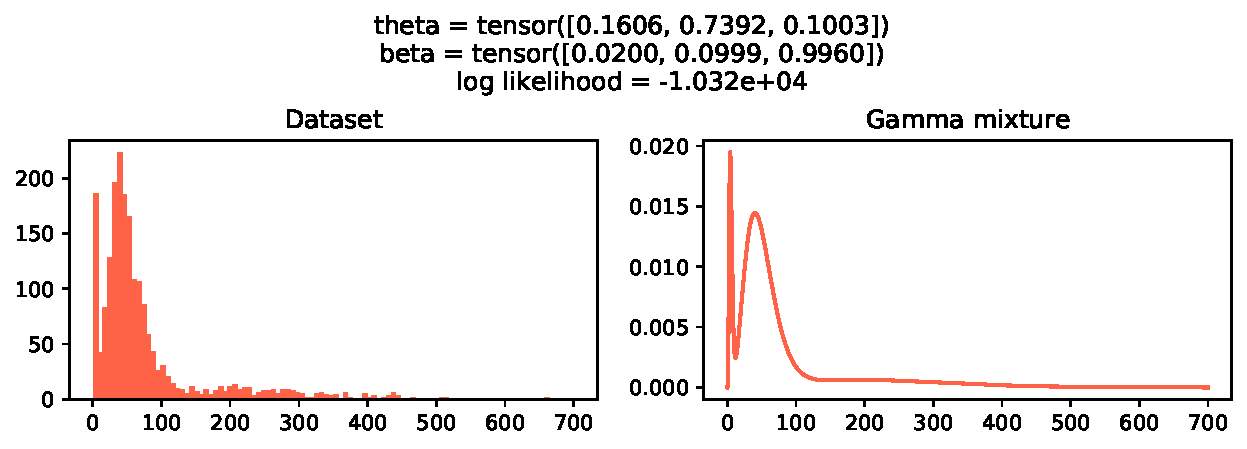
\includegraphics[width=\linewidth]{p1}

    Code:

    \begin{python}
def e_step(theta, betas):
    q = ds.Gamma(alpha, betas).log_prob(x) + torch.log(theta)
    q -= q.logsumexp(dim=1, keepdim=True)
    
    return q.exp()


def m_step(q):
    theta_hat = torch.sum(q, axis=0) / len(x)
    
    x_t = torch.transpose(x,0,1)
    beta_hats = alpha * torch.sum(q, axis=0) / torch.sum(torch.matmul(x_t, q), axis=0)

    return theta_hat, beta_hats


def log_px(x, theta, betas):
    p_gamma = ds.Gamma(alpha, betas).log_prob(x).exp()
    p = torch.sum(p_gamma * theta, axis=1)
    
    return p.log()


def run_em(theta, betas, iterations=1000):
    for _ in range(iterations):
        q = e_step(theta, betas)
        theta, betas = m_step(q)
        
    return theta, betas
    \end{python}
\end{enumerate}


\newpage

\begin{problem}[PCA, 15 pts]

% FDV: Here are the notes from last year.  I've already edited to make clear we want L2.  As noted below, we should also provide the baseline/reference to the pset 4 solutions in case they computed that wrong somehow.  
% 
% # problem 2 clarifications
% *NB: There was a lot of confusion about this problem, and we ended up accepting any form of comparison to PCA. Next year should clarify which norm students should use more explicitly (and maybe provide a baseline for students if the computation of the reconstruction error is different from what students calculated on pset4.)*
% 
% For Problem 2.3 (computing PCA reconstruction error), we will accept both the L1 and L2 norm and both summing over the errors for individual images and taking the mean of the errors (as long as you compute the error for K-Means the same way as you compute it for PCA). Apologies for the ambiguity in this question! 

  
For this problem you will implement PCA from scratch on the first 6000 images of the MNIST dataset. Your job is to apply PCA on MNIST and discuss what kind of structure is found. Implement your solution in \texttt{p2.ipynb} and attach the final plots below.

{\bfseries You will recieve no points for using third-party PCA implementations (i.e. {\normalfont \texttt{scikit-learn}}).}

{\bfseries You will recieve no points for code not included below.}
\begin{enumerate}

\item Compute the PCA. Plot the eigenvalues corresponding to the most
  significant 500 components in order from most significant to
  least. Make another plot that describes the cumulative proportion of
  variance explained by the first $k$ most significant components for
  values of $k$ from 1 through 500.  How much variance is explained by
  the first 500 components?  Describe how the cumulative proportion of
  variance explained changes with $k$.  Include this plot below.

\item Plot the mean image of the dataset and plot an image
  corresponding to each of the first 10 principle components.  How do
  the principle component images compare to the cluster centers from
  K-means? Discuss any similarities and differences.  Include these
  two plots below.

  \textit{Reminder: Center the data before performing PCA}

\item Compute the reconstruction error on the data set using the mean
  image of the dataset.  Then compute the reconstruction error using
  the first 10 principal components.  How do these errors compare to
  the final objective loss achieved by using K-means on the dataset?
  Discuss any similarities and differences.

  For consistency in grading, define the reconstruction error as the squared L2
  norm averaged over all data points.

\item Suppose you took the original matrix of principle components
  that you found $U$ and multiplied it by some rotation matrix $R$.
  Would that change the quality of the reconstruction error in the
  last problem?  The interpretation of the components?  Why or why
  not?
  
\end{enumerate}


\end{problem}

\newpage
\subsection*{Solution}
Plots:

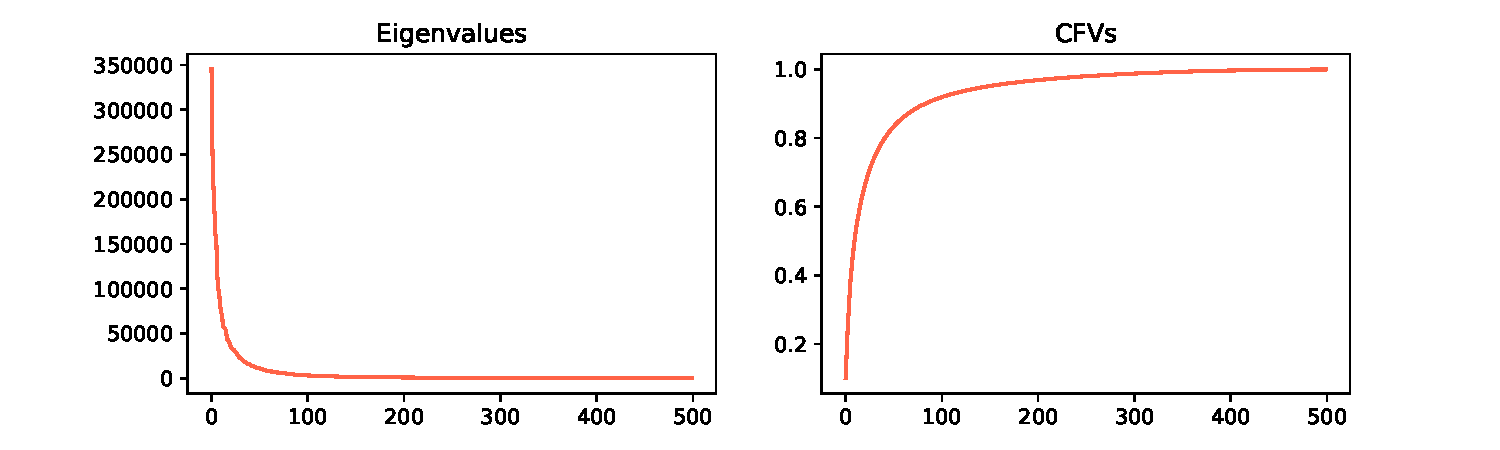
\includegraphics[width=\linewidth]{p2_cfvs}

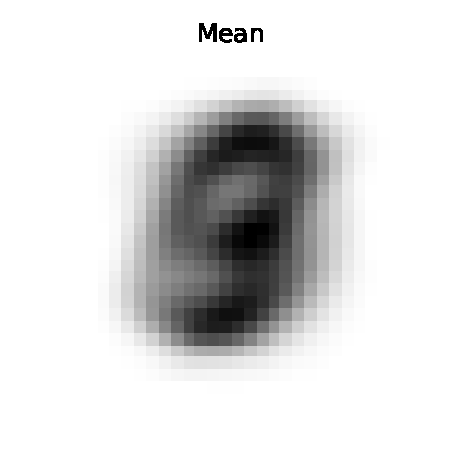
\includegraphics[width=0.25\linewidth]{p2_mean}
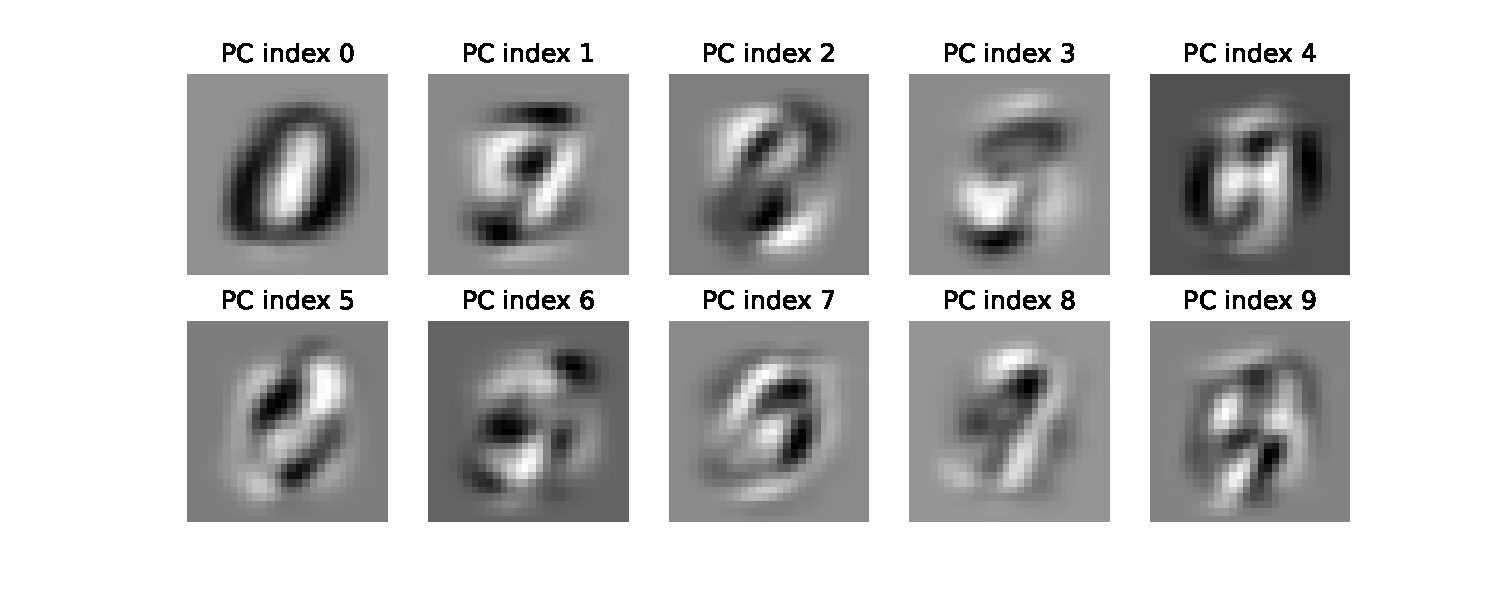
\includegraphics[width=0.75\linewidth]{p2_pcomps}

Code:

\begin{python}
# Standardize data
def standardize(x):
    mean = x.mean(0)
    x_std = (x - mean)
    return x_std

def pca(x, n_comps=500):

    x = standardize(x)

    U, S, V_t = torch.linalg.svd(x, full_matrices=False)

    S = torch.square(S) / N
    top_eigvals, top_indexes = torch.topk(S, n_comps)

    top_pcomps = V_t[top_indexes.tolist()]
    
    return top_eigvals, top_pcomps


def calc_cfvs(eigvals):
    cum_frac_vars = torch.cumsum(eigvals,0) / torch.sum(eigvals,0)
    return cum_frac_vars





def calc_errs(x, pcomps):
    x = standardize(x)

    err_mean = torch.linalg.norm(x, axis=1, ord=2)

    pcomps_matrix = torch.matmul(torch.transpose(pcomps[:10],0,1), pcomps[:10])
    err_pcomp = torch.linalg.norm(x - torch.matmul(x, pcomps_matrix), axis=1, ord=2)

    err_mean = err_mean.square().mean(0)
    err_pcomp = err_pcomp.square().mean(0)

    return err_mean, err_pcomp
\end{python}

\begin{enumerate}
  \item Almost all of the variance is explained by the first 500 components. As $k$ increases, the size of the eigenvalues decrease, and so the proportion of variance explained by the $k$th eigenvalue decreases. Thus, the cumulative proportion of variance explained is concave (down) as $k$ increases, i.e. increases less rapidly as $k$ increases.
  
  \item \quad\\
  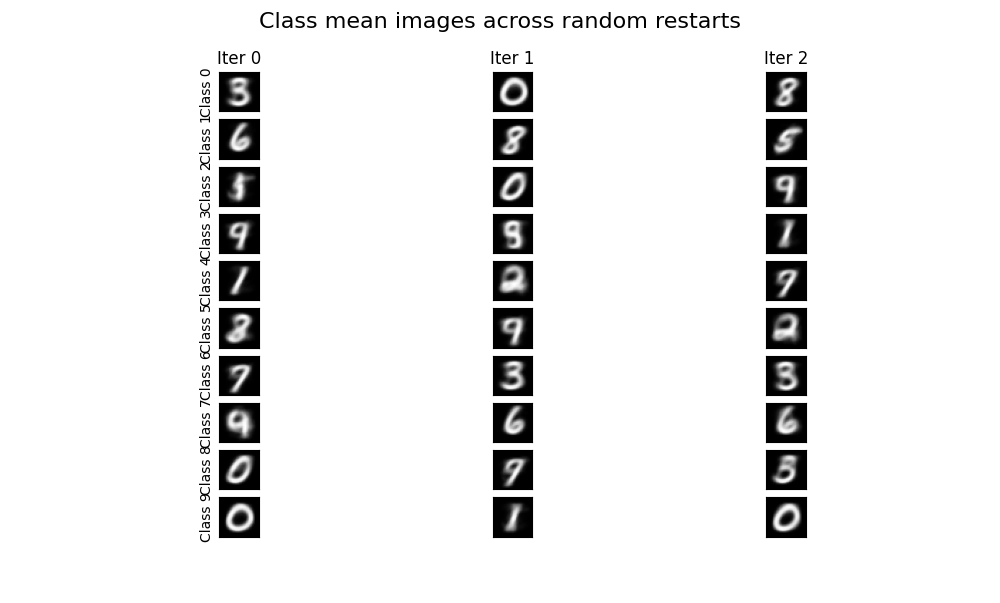
\includegraphics[width=0.75\linewidth]{HW4/2.2.png}\\
  K-means produces far sharper (less blurry) images than PCA. Intuitively, this makes sense as K-means works to cluster all the images in the same class (e.g. all of the 9s) and then averages the images in that cluster, such that the resulting centroid is a good prototype for images in that class (e.g. the cluster center looks like the average of many 9s as expected). By comparison, reconstructed images using PCA are blurrier because we lose spatial information by projecting the original images into a subspace with a lower dimension. As a result of having less information, reconstructed images could be really accurate, but they could also be really far away from what is the true clustering of identical images (e.g. ends up averaging reconstructed images that have very similar pixel values to real 9s, but also includes some images far away from the area in which there is a clustering of 9s). Thus, PCA gives us images that do not clearly distinguish between what is a number and what is a part of the background. Additionally, you can see that by averaging the different PCA images produced - i.e. creating a new linear combination of images - you could probably get closer to a sharper image (e.g. consider averaging PC index 2 and PC index 4 from the above in order to get a clearer 8). Thus, PCA does a good job but does not necessarily get its linear combinations right; K-means does a better job of producing clear images by placing them in the correct cluster, without having to weight them according to some linear combination, which it could get a bit wrong!
  
  In terms of similarities, it is clear that both PCA and K-means produce images that look like digits set on single-coloured backgrounds which have low variance. Although the backgrounds of the PCA images are lighter than the K-means images, background edge pixels have low variance across all the original images, so PCA and K-means are both able to re-produce this in the resulting images which all have a low variance across the background edge pixels.
  
  \item \quad
    \begin{center}
        \begin{tabular}{ |c|c| } 
        \hline
        Reconstruction error (using mean) & $3.436022 \times 10^6$ \\
        \hline
        Reconstruction error (using mean and top 10 pcomps) & $1.731315 \times 10^6$\\
        \hline
        K-means objective loss & $1.3 \times 10^10$\\
        \hline
        \end{tabular}
    \end{center}
    The loss calculated from my implementation of K-means (in the table above) is not well suited for this comparison (it should be c. $2.6 \times 10^6$ - from office hours). We would expect the K-means loss to be between the reconstruction errors with and without using the principal components. Clearly, the reconstruction error using the mean should be the highest, since we are not doing any machine learning, just finding the squared loss between every image and the average of all the images. (If we had an algorithm that did worse than this, we would have wasted a lot of time!) The reconstruction error  using the top 10 principal components should be the lowest because we know that the PCA algorithm minimizes the reconstruction error by projecting into a lower subspace using the principal components. By comparison, K-means should have a slightly higher loss (albeit still lower than the reconstruction error, not using the principal components) since it is placing images into clusters and then taking averages of those clusters. The loss compares the original images with these averages, which are arguably just more sophisticated averages than the one average of all the data used by the reconstruction error, not using the principal components. Thus, K-means gets us a local minimum ob the objective function, iterating in such a way that the loss always decreases, but never minimizing the objective function to the same extent as PCA with its reconstruction loss using the principal components.

  \item Multiplying $U$ by some rotation matrix $R$ would not change the quality of the reconstruction error, since the eigenvectors in $U$ define an orthogonal basis of the lower dimensional subspace, from which we are reconstructing the data. Rotating all of these eigenvectors still results in an orthogonal basis that defines this same subspace, and so we can still reconstruct the images using a linear combination of these rotated eigenvectors. However, the interpretation of these rotated components changes as they no longer point in the directions of maximum variance.
\end{enumerate}

\newpage

\begin{problem}[Bayesian Networks, 10 pts]

% FDV: I think we can keep this problem as-is, and just clarfiy based
% on notes from last year.
% # problem 3 clarifications
% The phrasing of Q3 is slightly off because it implies that you need to explain why each path is not blocked in the case that two nodes are not independent. It is sufficient to provide a single unblocked path. Better phrasing is (emphasis added) "Use the concept of d-separation to answer the questions and show your work (i.e., state what the blocking path(s) is/are and which node blocks the path; or explain why there exists a path that is not blocked)." 
% 
% Some helpful resources for d-separation:  The 2020 Section 8 notes, Bishop p. 372 - 379, Section 8.2 of the CS 181 textbook
% 
% Problem 3: Make it clear (put the instructions in one place) that we require explanations for both "yes" and "no" answers

  
  \noindent In this problem we explore the conditional independence
  properties of a Bayesian Network.  Consider the following Bayesian
  network representing a fictitious person's activities. Each random
  variable is binary (true/false).

\begin{center}
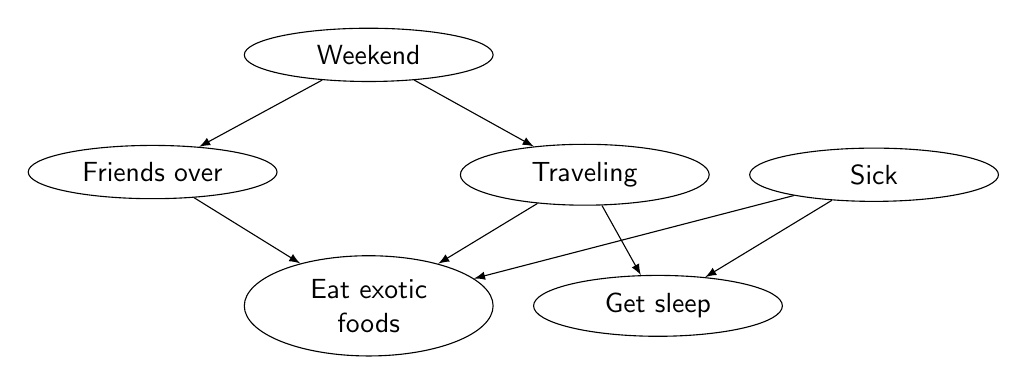
\begin{tikzpicture}[
  node distance=1cm and .5cm,
  bn/.style={draw,ellipse,text width=2cm,align=center}
    ]
    \node[bn] (w) {\attr{Weekend}};
    \node[bn,below right=of w] (t) {\attr{Traveling}};
    \node[bn,right=of t] (s) {\attr{Sick}};
    \node[bn,below left=of w] (f) {\attr{Friends over}};
    \node[bn,below right=of f] (eef) {\attr{Eat exotic foods}};
    \node[bn,right=of eef] (gs) {\attr{Get sleep}};
    \path (w) edge[-latex] (t)
    (w) edge[-latex] (f)
    (f) edge[-latex] (eef)
    (t) edge[-latex] (eef)
    (t) edge[-latex] (gs)
    (s) edge[-latex] (gs)
    (s) edge[-latex] (eef);
    \end{tikzpicture}
\end{center}

The random variables are:

\begin{itemize}
\item \attr{Weekend}: Is it the weekend?
\item \attr{Friends over}: Does the person have friends over?
\item \attr{Traveling}: Is the person traveling?
\item \attr{Sick}: Is the person sick?
\item \attr{Eat exotic foods}: Is the person eating exotic foods?
\item \attr{Get Sleep}: Is the person getting sleep?
\end{itemize}

\medskip

For the following questions, $A \perp B$ means that events A and B are
independent and $A \perp B | C$ means that events A and B are independent
conditioned on C.

\textbf{Use the concept of d-separation} to answer the
questions and show your work (i.e., state what the blocking path(s) is/are and what nodes block the path; or explain why each path is not blocked).

\textit{Example Question:} Is $\attr{Friends over} \perp \attr{Traveling}$? If NO, give intuition for why.

\textit{Example Answer:} NO. The path from Friends over -- Weekend -- Traveling is not blocked following the d-separation rules as we do not observe Weekend. Thus, the two are not independent. 

\textbf{Actual Questions:}

\begin{enumerate}
\item Is $\attr{Weekend} \perp \attr{Get Sleep}$?
  If NO, give intuition for why.

\item Is $\attr{Sick} \perp \attr{Weekend}$?
  If NO, give intuition for why.


\item Is $\attr{Sick} \perp \attr{Friends over}\given \attr{Eat exotic
  foods}$? If NO, give intuition for why.


\item Is $\attr{Friends over} \perp \attr{Get Sleep}$? If NO, give
  intuition for why.

\item Is $\attr{Friends over} \perp \attr{Get Sleep} \given
  \attr{Traveling}$? If NO, give intuition for why.

\item Suppose the person stops traveling in ways that affect their
  sleep patterns.  Travel still
  affects whether they eat exotic foods.  Draw the modified network. (Feel free to reference the handout file for the commands for displaying the new network in \LaTeX).

\item For this modified network, is $\attr{Friends over} \perp
  \attr{Get Sleep}$? If NO, give an intuition why.  If YES,
  describe what observations (if any) would cause them to no longer be
  independent.

\end{enumerate}
\end{problem}

\newpage
\section*{Solution}
\begin{enumerate}
  \item NO. The path from Weekend -- Traveling -- Get sleep is not blocked following the d-separation rules as we do not observe Traveling. Thus, the two are not independent.
  \item YES. The path from Sick -- Get sleep -- Traveling -- Weekend is blocked following the d-separation rules as we do not observe Get Sleep. The other path from Sick -- Eat exotic foods -- Friends over -- Weekend is blocked following the d-separation rules as we do not observe Eat exotic foods. Thus, the two are independent.
  \item NO. The path from Sick -- Eat exotic foods -- Friends over is not blocked following the d-separation rules as we now observe Eat exotic foods. Thus, the two are not independent given Eat exotic foods.
  \item NO. The path from Get sleep -- Traveling -- Weekend -- Friends over is not blocked following the d-separation rules as we do not observe Traveling nor Weekend. Thus, the two are not independent.
  \item YES. The path from Get sleep -- Traveling -- Weekend -- Friends over is blocked following the d-separation rules as we now observe Traveling. Likewise, the other path from Get sleep -- Traveling -- Eat exotic foods -- Friends over is blocked following the d-separation rules by observing Traveling. Finally, the path from Get sleep -- Sick -- Eat exotic foods -- Friends over is blocked following the d-separation rules as we do not observe Eat exotic foods. Thus, the two are independent given Traveling. 
  \item \quad
  
      \begin{center}
        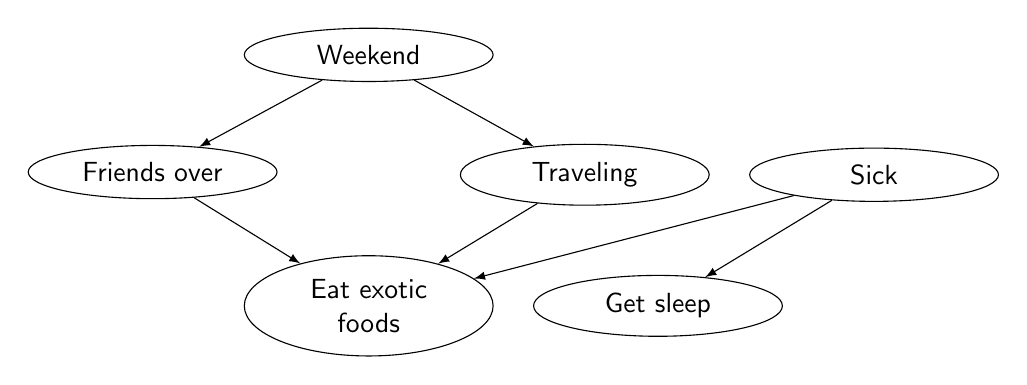
\begin{tikzpicture}[
          node distance=1cm and .5cm,
          bn/.style={draw,ellipse,text width=2cm,align=center}
            ]
            \node[bn] (w) {\attr{Weekend}};
            \node[bn,below right=of w] (t) {\attr{Traveling}};
            \node[bn,right=of t] (s) {\attr{Sick}};
            \node[bn,below left=of w] (f) {\attr{Friends over}};
            \node[bn,below right=of f] (eef) {\attr{Eat exotic foods}};
            \node[bn,right=of eef] (gs) {\attr{Get sleep}};
            \path (w) edge[-latex] (t)
            (w) edge[-latex] (f)
            (f) edge[-latex] (eef)
            (t) edge[-latex] (eef)
            (s) edge[-latex] (gs)
            (s) edge[-latex] (eef);
            \end{tikzpicture}
        \end{center}

  \item YES. The path from Get sleep -- Sick -- Eat exotic foods -- Friends over is blocked following the d-separation rules as we do not observe Eat exotic foods. Thus, the two are independent.
\end{enumerate}

\newpage
%%%%%%%%%%%%%%%%%%%%%%%%%%%%%%%%%%%%%%%%%%%%%
% Name and Calibration
%%%%%%%%%%%%%%%%%%%%%%%%%%%%%%%%%%%%%%%%%%%%%
\subsection*{Name}
Ben Ray

\subsection*{Collaborators and Resources}
Whom did you work with, and did you use any resources beyond cs181-textbook and your notes?\\
CS 181 Office Hours\\
Ty Geri\\
Josh Michels\\
\subsection*{Calibration}
Approximately how long did this homework take you to complete (in hours)?\\
14

\end{document}
